\documentclass[12pt]{article}

\usepackage[utf8]{inputenc}
\usepackage[polish]{babel}
\usepackage[T1]{fontenc}
\usepackage{indentfirst}
\usepackage{polski}
\usepackage{graphicx} 
\usepackage{float}
\usepackage{color}   %May be necessary if you want to color links
\usepackage{hyperref}
\usepackage{subfig} %obrazki obok siebie
\usepackage{spverbatim}  %for code snippets


\usepackage{listings}
\usepackage{color}

\definecolor{dkgreen}{rgb}{0,0.6,0}
\definecolor{gray}{rgb}{0.5,0.5,0.5}
\definecolor{mauve}{rgb}{0.58,0,0.82}

\lstset{frame=tb,
	language=C,
	aboveskip=3mm,
	belowskip=3mm,
	showstringspaces=false,
	columns=flexible,
	basicstyle={\small\ttfamily},
	numbers=none,
	numberstyle=\tiny\color{gray},
	keywordstyle=\color{blue},
	commentstyle=\color{dkgreen},
	stringstyle=\color{mauve},
	breaklines=true,
	breakatwhitespace=true,
	tabsize=3
}
\hypersetup{
    colorlinks=true, %set true if you want colored links
    linktoc=all,     %set to all if you want both sections and subsections linked
    linkcolor=black,  %choose some color if you want links to stand out
}

\graphicspath{{img/}}



\usepackage[top=2cm, bottom=2cm, left=3cm, right=3cm]{geometry}
\makeatletter
\newcommand{\linia}{\rule{\linewidth}{0.4mm}}
\renewcommand{\maketitle}{\begin{titlepage}
		\vspace*{1cm}
		\begin{center}\small
			Poliechnika Śląska\\
			Wydział Automatyki, Elektroniki i Informatyki\\
			Raport Zarządzanie Projektami
		\end{center}
		\vspace{3cm}
		\noindent\linia
		\begin{center}
			\LARGE \textsc{\@title}
		\end{center}
		\linia
		\vspace{0.5cm}
		\begin{flushright}
			\begin{minipage}{15cm}
				\textit{\small Autorzy:}\\
				\normalsize \textsc{Kamil Choiński} \par \textsc{Oskar Stabla} \par
			\end{minipage}	
		\end{flushright}
		\vspace*{\stretch{6}}
		\begin{center}
			\@date
		\end{center}
	\end{titlepage}
}
\makeatother

\title{Plantie™}




\begin{document}
	
\maketitle

\tableofcontents

\newpage

\section{Karta projektu}


\subsection{Cele projektu}
Nasz projekt ma na celu pomóc zabieganym ludziom, którzy nie mają czasu na zajmowanie się
swoją roślinką przez swój częsty brak pobytu w domu. Wystarczy dostęp do internetu,
nic więcej.

Powstała koncepcja opiera się na systemie zdalnego zarządzania rośliną. Chcemy mierzyć parametry
gleby i otoczenia takie jak wilgotność, nasłonecznienie, a nawet poziom wody w zbiorniku do podlewania. W zależności od odczytanych wartości przez
płytkę rozwojową UNO połączoną z modułem ESP8266, będzie możliwe sterowanie pompką wody i oświetleniem rośliny. Postanowiliśmy utworzyć panel sterowania na stronie
internetowej.

\subsection{Produkty projektu}



\begin{itemize}
	\item Zespół urządzeń akwizycyjno-wykonawczych  
	\item Panel sterowania na stronie internetowej 
	\item Aplikacja mobilna 
\end{itemize}

\subsection{Uproszczony harmonogram}


\subsubsection{Miesiąc 1}
Pomysł, przegląd podobych rozwiązań dostępnych na rynku.
Próba dopasowania się do konkurencji z własnym rozwiązaniem.

Przeanalizowanie współpracy płytki rozwojowej UNO, modułu komunikacyjnego ESP8266, czujnika wilgotności gleby, czujnika wilgotności powietrza i czujnika nasłonecznienia oraz rozwiązanie techniczne doświetlania rośliny. 

\subsubsection{Miesiąc 2}

Stworzenie schematu elektrycznego projektu. Testowanie poprawności działania posiadanych czujników w warunkach domowych. Implementacja komunikacji z modułem ESP8266. Dopasowywanie czasów działania.

Równoczesne tworzenie aplikacji zajmującej się zarządzaniem zapytaniami i realizującej funkcję komunikacji z użytkownikiem opartej o websocket. Tworzenie aplikacji zajmującej się identyfikacją rodzaju rośliny.

\subsubsection{Miesiąc 3}
Realizacja połączeń elektrycznych na płytce stykowej i ostateczne testowanie poprawności działania aplikacji. Realizacja montażu systemu doświetlania. Przeniesienie projektu na płytkę uniwersalną i zaprojektowanie własnej płytki.

Połączenie systemu wykrywania rośliny i systemu zarządzania.


\subsubsection{Miesiąc 4}

Przygotowanie obudowy i instrukcji użytkowania. 

Planowanie i realizacja produkcji. 

\subsubsection{Miesiąc 5}
Testowanie produktu przez użytkowników pre-orderowych, marketing.
Ostateczne poprawy błędów.
Prezentacja gotowego projektu.





\subsection{Budżet projektu}


\begin{table}[!h]
	\centering
	\begin{tabular}{l|r}
		Komponent projektu & Cena \\\hline
		
		Części do testów & 1 000 PLN \\
		
		Wynajem biura & 15 000 PLN \\
		
		Licencje oprogramowania & 5 000 PLN \\
		
		Wynagrodzenie dla specjalistów & 150 000 PLN \\
		
		Marketing & 10 000 PLN \\
		
		Produkcja i koszty magazynowania & 50 000 PLN \\
		
		\hline
		Suma & 231 000 PLN
		
	\end{tabular}
	
\end{table}

Same komponenty projektu zostaną sprowadzone z Chin.



\subsection{Uproszczony opis zespołu projektowego}

\begin{itemize}
	
\item Stefan (35zł/h) - Team lead, odpowiedzialny za organizację pracy zespołu

\item Janusz (25zł/h) - Marketing manager, odpowiedzialny za marketing 

\item Jeff (24zł/h) - Elektronik, odpowiedzialny za układy cyfrowe

\item Kamil (22zł/h) - Mechanik/Web Designer, odpowiedzialny za projekt strony i nadzór konstrukcji obudowy

\item Oskar (26zł/h) - Programista wysokopoziomowy, odpowiedzialny za software od strony serwerowej do systemu przetwarzania danych

\item Tomasz (26zł/h) - Programista aplikacji mobilnych i systemu przetwarzania informacji wizyjnych

\item Krzysztof (19zł/h) - Logistyk 

\end{itemize}


\newpage
\section{Opis merytoryczny}

\subsection{Stan wiedzy w dziedzinie objętej projektem - podobne projekty}


\subsubsection{Trutina}
‘Trutina’ z Gremon Systems przedstawiony na Rysunku nr \ref{fig:Trutina},
 pozwala na automatyczne podlewanie danej rośliny, a także na pomiary parametrów za pomocą sensorów wbudowanych w urządzenie takich jak: pyranometer, E-box, GS3 które wysyłając pomiary, kontroluje system i wybiera kiedy podlać roślinę. 

System posiada także aplikację na telefon, dzięki której możemy podglądać graficznie mierzone parametry, a także kontrolować system podlewający. 


Różni sie od naszego projektu aplikacją, gdyż otrzymujemy wszystkie pomiary na stronie internetowej i samoistnym wyborem kiedy będzie włączone podlewanie. Jest to także dużo większy projekt od naszego gdyż jest przystosowany do pracy w warunkach terenowych, nasz zaś do domowych.



\begin{figure}[!h]
	\begin{center}
		{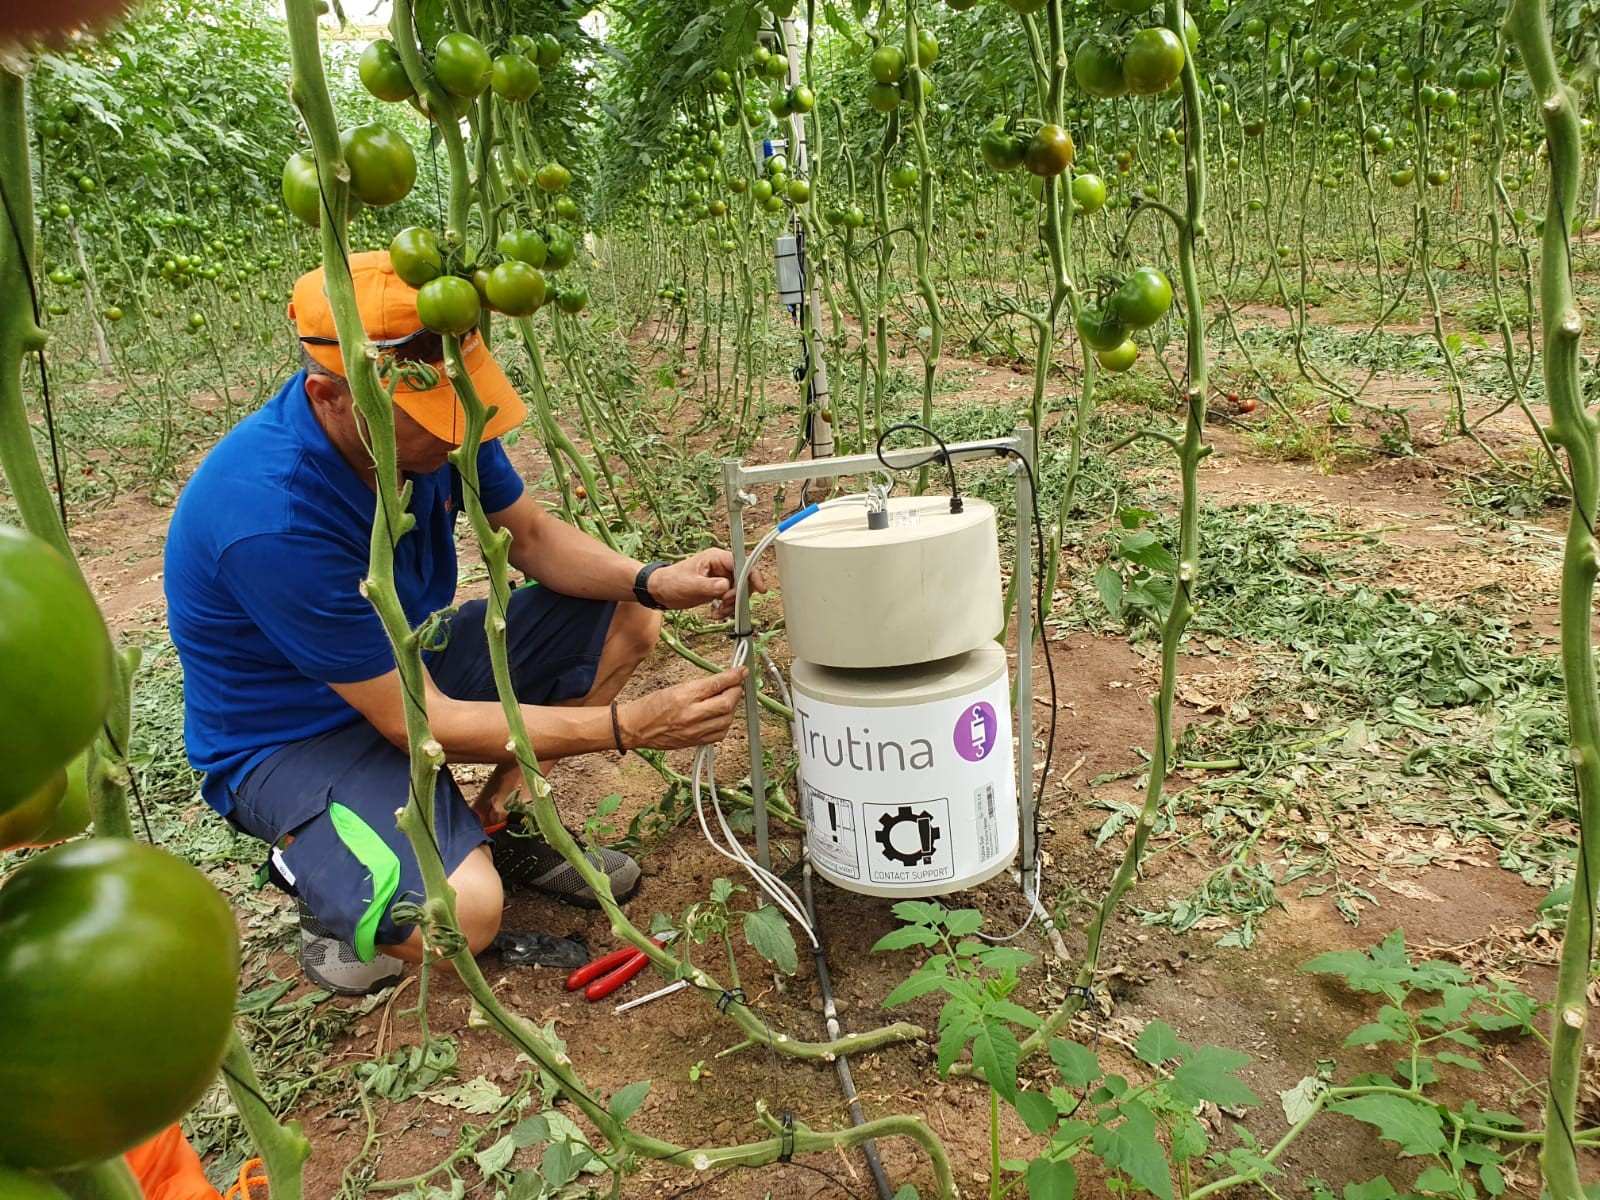
\includegraphics[width=10cm]{auto_water1.jpg}}
	\end{center}
	\caption{Trutina ~\cite{Trutina}}
	\label{fig:Trutina}
\end{figure}


\newpage
\subsubsection{Arduino Irrigator System }

Ten projekt przedstawiony na Rysunku nr \ref{fig:ArduinoIS}, bazuje na płytce rozwojowej Arduino UNO i ma na celu automatyzację procesu pomiarów parametrów rośliny i jej podlewaniu. System bada wilgotność gleby i włącza pompę wodną jeśli wilgotność spadnie poniżej pewnego poziomu. Kiedy system wykryje wartość powyżej ustalonej wyłączy pompę. System posiada także wyświetlacz LCD 16x2 na którym są wyświetlane: poziom wody w zbiorniku, status czy pompka jest włączona, wilgotność gleby.

Projekt różni się od naszego sposobem wyświetlania danych - różnica wyświetlaczy, a także brakiem zapisywania pomiarów i połączeniem z siecią Wi-Fi.



\begin{figure}[!h]
	\begin{center}
		{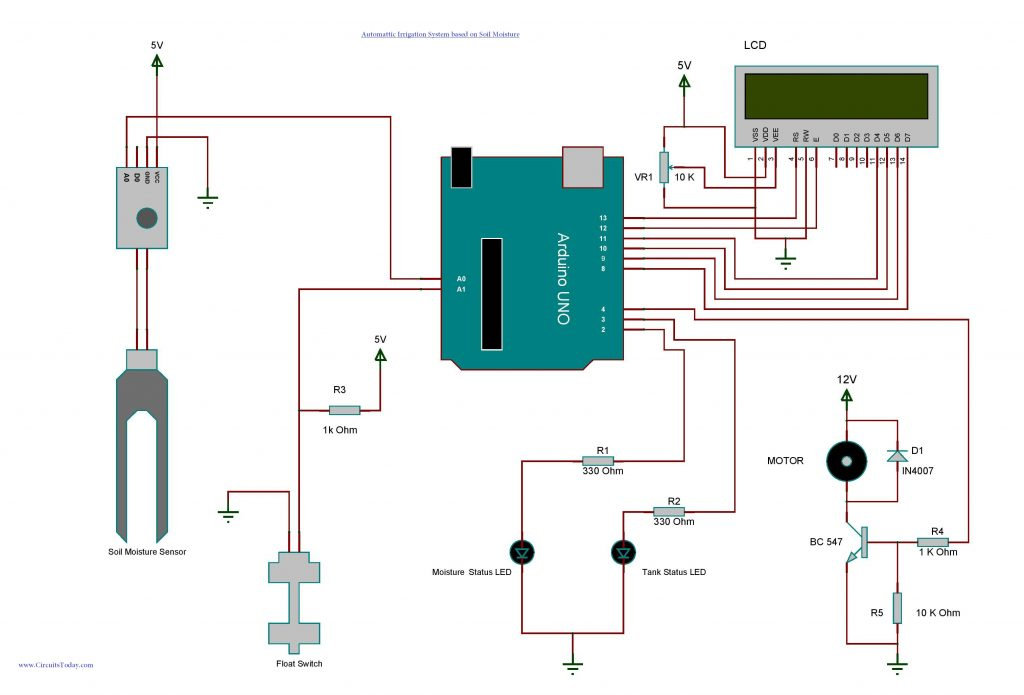
\includegraphics[width=8cm]{arduino_przyklad2.jpg}}
	\end{center}
	\caption{Arduino Irrigator System ~\cite{ArduinoIS}}
	\label{fig:ArduinoIS}
\end{figure}




\subsection{Opis działań przeznaczonych do realizacji }

\begin{itemize}
	\item Zebranie drużyny projektowej
	
	\item Przegląd dostępnych rozwiązań
	
	\item Dopasowanie do rynku
	\item Realizacja projektu
	\item Marketing 
\end{itemize}



\subsection{Uzasadnienie innowacyjności podjętych działań }


Nasz produkt oferuje możliwość rozpoznawania rodzaju rośliny poprzez przesłanie zdjęcia jej liścia do osobnej aplikacji zajmującej się identyfikacją. Dzięki temu możliwe jest dopasowanie harmonogramu podlewania i doświetlania w zależności od wymagań danej rośliny.

\subsection{Spodziewany efekt }


Przyjecie produktu przez rynek, zadowolenie konsumenta.
 
Wykup projektu przez większą firmę.




%coś z tego do wpierdolenia wyżej
%Przed rozpoczęciem prac nad projektem utworzyliśmy tabele w programie internetowym Trello, na których zapisaliśmy rzeczy potrzebne do zrobienia, a także podział kto jakimi elementami projektu się zajmie. Najtrudniejszą częścią wydawała nam się implementacja połączeń pomiędzy płyką rozwojową UNO, ESP8266 oraz serwerem, więc postanowiliśmy zacząć od tego, a dopiero później przejść do następnych aspektów. Wyzwaniem dla nas była również współpraca nad tak rozległym projektem, w którym wymagane było poprawne i integralne działanie zarówno części hardware'u, jak i tej internetowej. Zdecydowanie z pomocą przyszedł nam GitHub, ułatwiający zarówno równoległą pracę, jak i ewentualne poprawy błędów. 
%Ku naszemu zdziwieniu, projekt zajął zdecydowanie więcej czasu niż mogliśmy się spodziewać. Brak wiedzy skutkował tym, że nie wiedzieliśmy nawet gdzie i czego szukać. Na szczęście internet w dzisiejszych czasach jest bardzo obszerny w różnego rodzaju poradniki i źródła, które pomogły nam zrealizować cele i wyjaśnić czemu poprzednie próby musiały zakończyć się fiaskiem. 
%
%Podsumowując, jesteśmy bardzo zadowoleni z ogólnego rezultatu. Niestety, nie wszystko poszło zgodnie z planem, lecz połączenie rozwiązań technicznych i cyfrowych oraz sprawienie, by działały wspólnie spowodowały powstanie ciekawego dla nas projektu oraz zdobycie bardzo cennej wiedzy. Realizacja własnego projektu mikroprocesorowego, który zmusza do samodzielnego myślenia, swoboda w jego tworzeniu oraz doprowadzenie całości do finalnego produktu jest z pewnością bardzo satysfakcjonująca i pomimo czasu, który trzeba w to włożyc, powinno być ich więcej.
%\subsection{Pomysły na rozwój projektu}
%Pomysłów na dalszy rozwój projektu jest wiele, ponieważ w trakcie prac przychodziło nam do głowy ich dużo jednak postanowiliśmy je tymczasowo zignorować i spróbować zrealizować postawione przez nas na początku cele. Nie zrealizowaliśmy również jednego aspektu projektu co też stało się naszym planem na przyszłość. \\







%
%\section{Szczegółowy opis projektu}
%
%
%\subsection{Rozwiązania techniczne - Przegląd modułów projektu}
%\subsubsection{Czujnik wilgotności i temperatury powietrza: DHT11}
%Pomiary wilgotności i temperatury powietrza są wykonywane z użyciem czujnika DHT11. Do implementacji w ArduinoIDE została wykorzystana biblioteka DHT-sensor-library, aby pomiary wykonywały się poprawnie, dzięki czemu ręczna kalibracja nie była potrzebna. Czujnik przedstawiony na Rysunku nr \ref{fig:dht11}.
%\begin{figure}[!h]
%	\begin{center}
%		{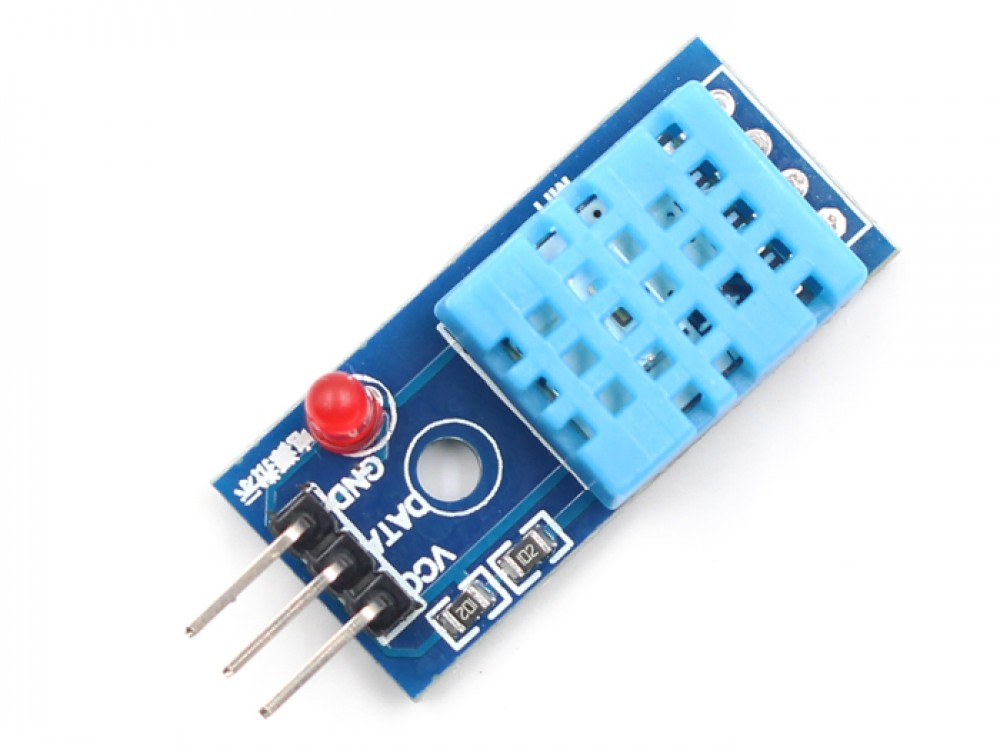
\includegraphics[width=5cm]{DHT11_photo.png}}
%	\end{center}
%	\caption{Czujnik DHT11}
%	\label{fig:dht11}
%\end{figure}
%
%
%\newpage
%\subsubsection{Czujnik natężenia światła}
%Pomiary natężenia aktualnego oświetlenia w otoczeniu rośliny są wykonywane z użyciem czujnika natężenia światła. Jego parametry były skonfigurowane na podstawie własnych doświadczeń: 0 procent - czujnik zakryty ciemnym materiałem, 100 procent - czujnik oświecony mocnym źródłem światła. Czujnik przedstawiony na Rysunku nr \ref{fig:Czujnikswiatla}.
%\begin{figure}[!h]
%	\begin{center}
%		{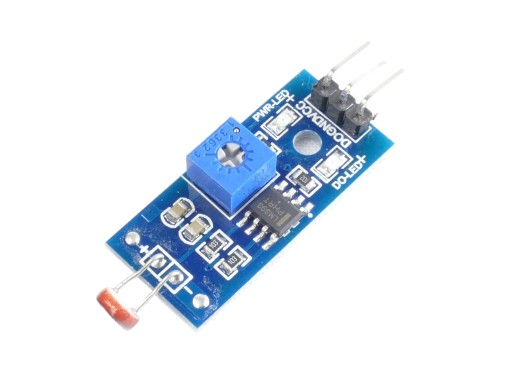
\includegraphics[width=7cm]{light_sensor_photo.png}}
%	\end{center}
%	\caption{Czujnik natężenia światła}
%		\label{fig:Czujnikswiatla}
%\end{figure}
%\subsubsection{Czujnik wilgotności gleby FC-28}
%Pomiary wilgotności gleby naszej rośliny są wykonywane z użyciem czujnika wilgotności gleby FC-28. Jego parametry były skonfigurowane na podstawie własnych doświadczeń: 0 procent - czujnik w powietrzu - brak powierzchni styku, 100 procent - czujnik zanurzony w wodzie. Czujnik przedstawiony na Rysunku nr \ref{fig:28}.
%
%\begin{figure}[!h]
%	\begin{center}
%		{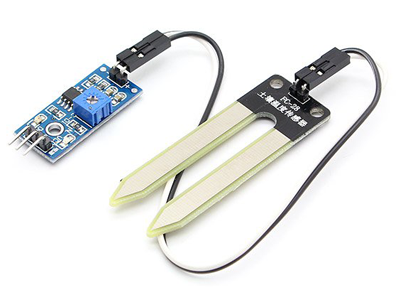
\includegraphics[width=7cm]{FC-28_photo.png}}
%	\end{center}
%	\caption{Czujnik FC-28}
%	\label{fig:fc28}
%\end{figure}
%
%\newpage
%\subsubsection{Czujnik poziomu wody w zbiorniku}
%Pomiary aktualnego poziomu wody w zbiorniku z wodą do podlewania są wykonywane z użyciem czujnika poziomu wody. Jego parametry były skonfigurowane na podstawie własnych doświadczeń: 0 procent - czujnik suchy, nie zanurzony w wodzie, 100 procent - czujnik w całości zanurzony w wodzie. Czujnik przedstawiony na Rysunku nr \ref{fig:waterlevel}.
%\begin{figure}[!h]
%	\begin{center}
%		{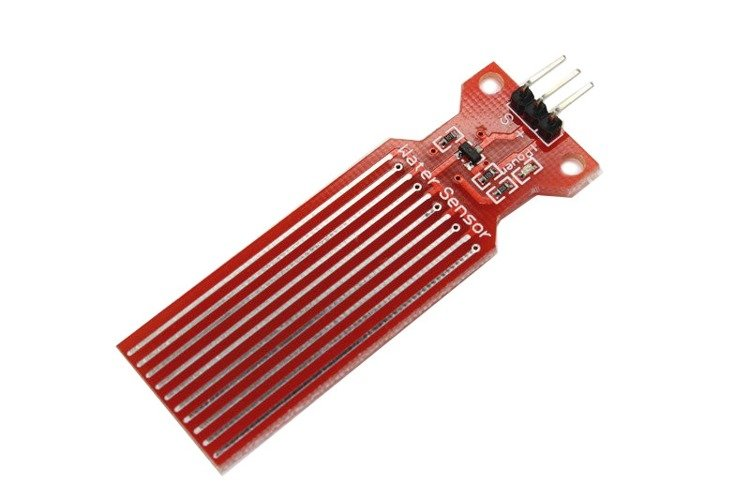
\includegraphics[width=6cm]{water_sensor_photo.png}}
%	\end{center}
%	\caption{Czujnik poziomu wody}
%	\label{fig:waterlevel}
%\end{figure}
%
%\subsubsection{Wyświetlacz OLED}
%Zewnętrzne wyświetlanie pomiarów wilgotności gleby i powietrza jest obsługiwane przez wyświetlacz OLED zamontowany na przodzie obudowy, aby była możliwość monitorowania jej stanu, gdy przebywamy w jej otoczeniu bez potrzeby połączenia internetowego. Do poprawnego wyświetlania danych na ekranie zostały wykorzystane biblioteki AdafruitGFX.h i AdafruitSSD1306.h.
%Wyświetlacz przedstawiony na Rysunku nr \ref{fig:oled}.
%\begin{figure}[!h]
%	\begin{center}
%		{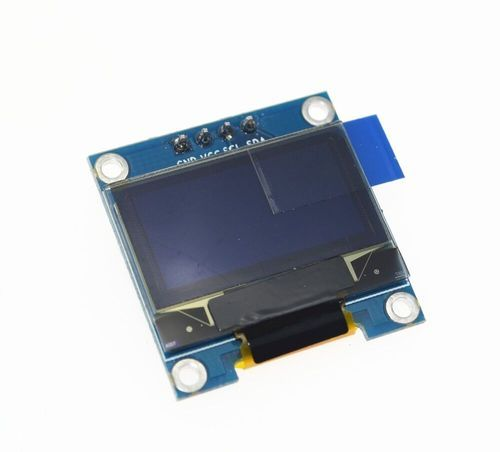
\includegraphics[width=8cm]{oled-display_photo.png}}
%	\end{center}
%	\caption{0.96 calowy wyświetlacz OLED}
%	\label{fig:oled}
%\end{figure}
%
%\subsubsection{Przekaźnik, Pompka wodna}
%Do układu została zamontowana samochodowa pompka do spyskiwaczy firmy TOPRAN, gdyż było to tańsze rozwiązanie niż inne rodzaje pompek. Jej napięcie znamionowe wynosi 12 [V], jednak w projekcie do jej zasilania używamy baterii 9 [V], które w zupełności spełnia wymagania stawiane przez dotyczące jej wydajności. Okresowe zasilanie jest realizowane za pomocą przekaźnika, do którego z jednej strony wpięta jest bateria i pompka, a z drugiej zasilanie 5 [V] z płytki rozwojowej UNO zasilające sam przekaźnik, GND i sygnał sterujący. Komponenty przedstawione na Rysunku nr \ref{fig:komponenty}.
%
%
%
%
%\begin{figure}[!h]
%%%obrazki
%\centering
%\subfloat[Przekaźnik~\cite{przekaznik}]{\label{odnosnik}
%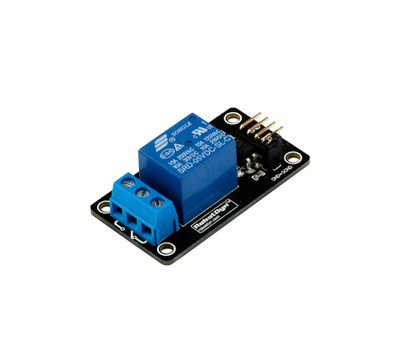
\includegraphics[width=0.4\textwidth]{Przekaznik_photo.jpg}}
%\quad
%\subfloat[Pompa wodna~\cite{pompka}]{\label{odnosnik}
%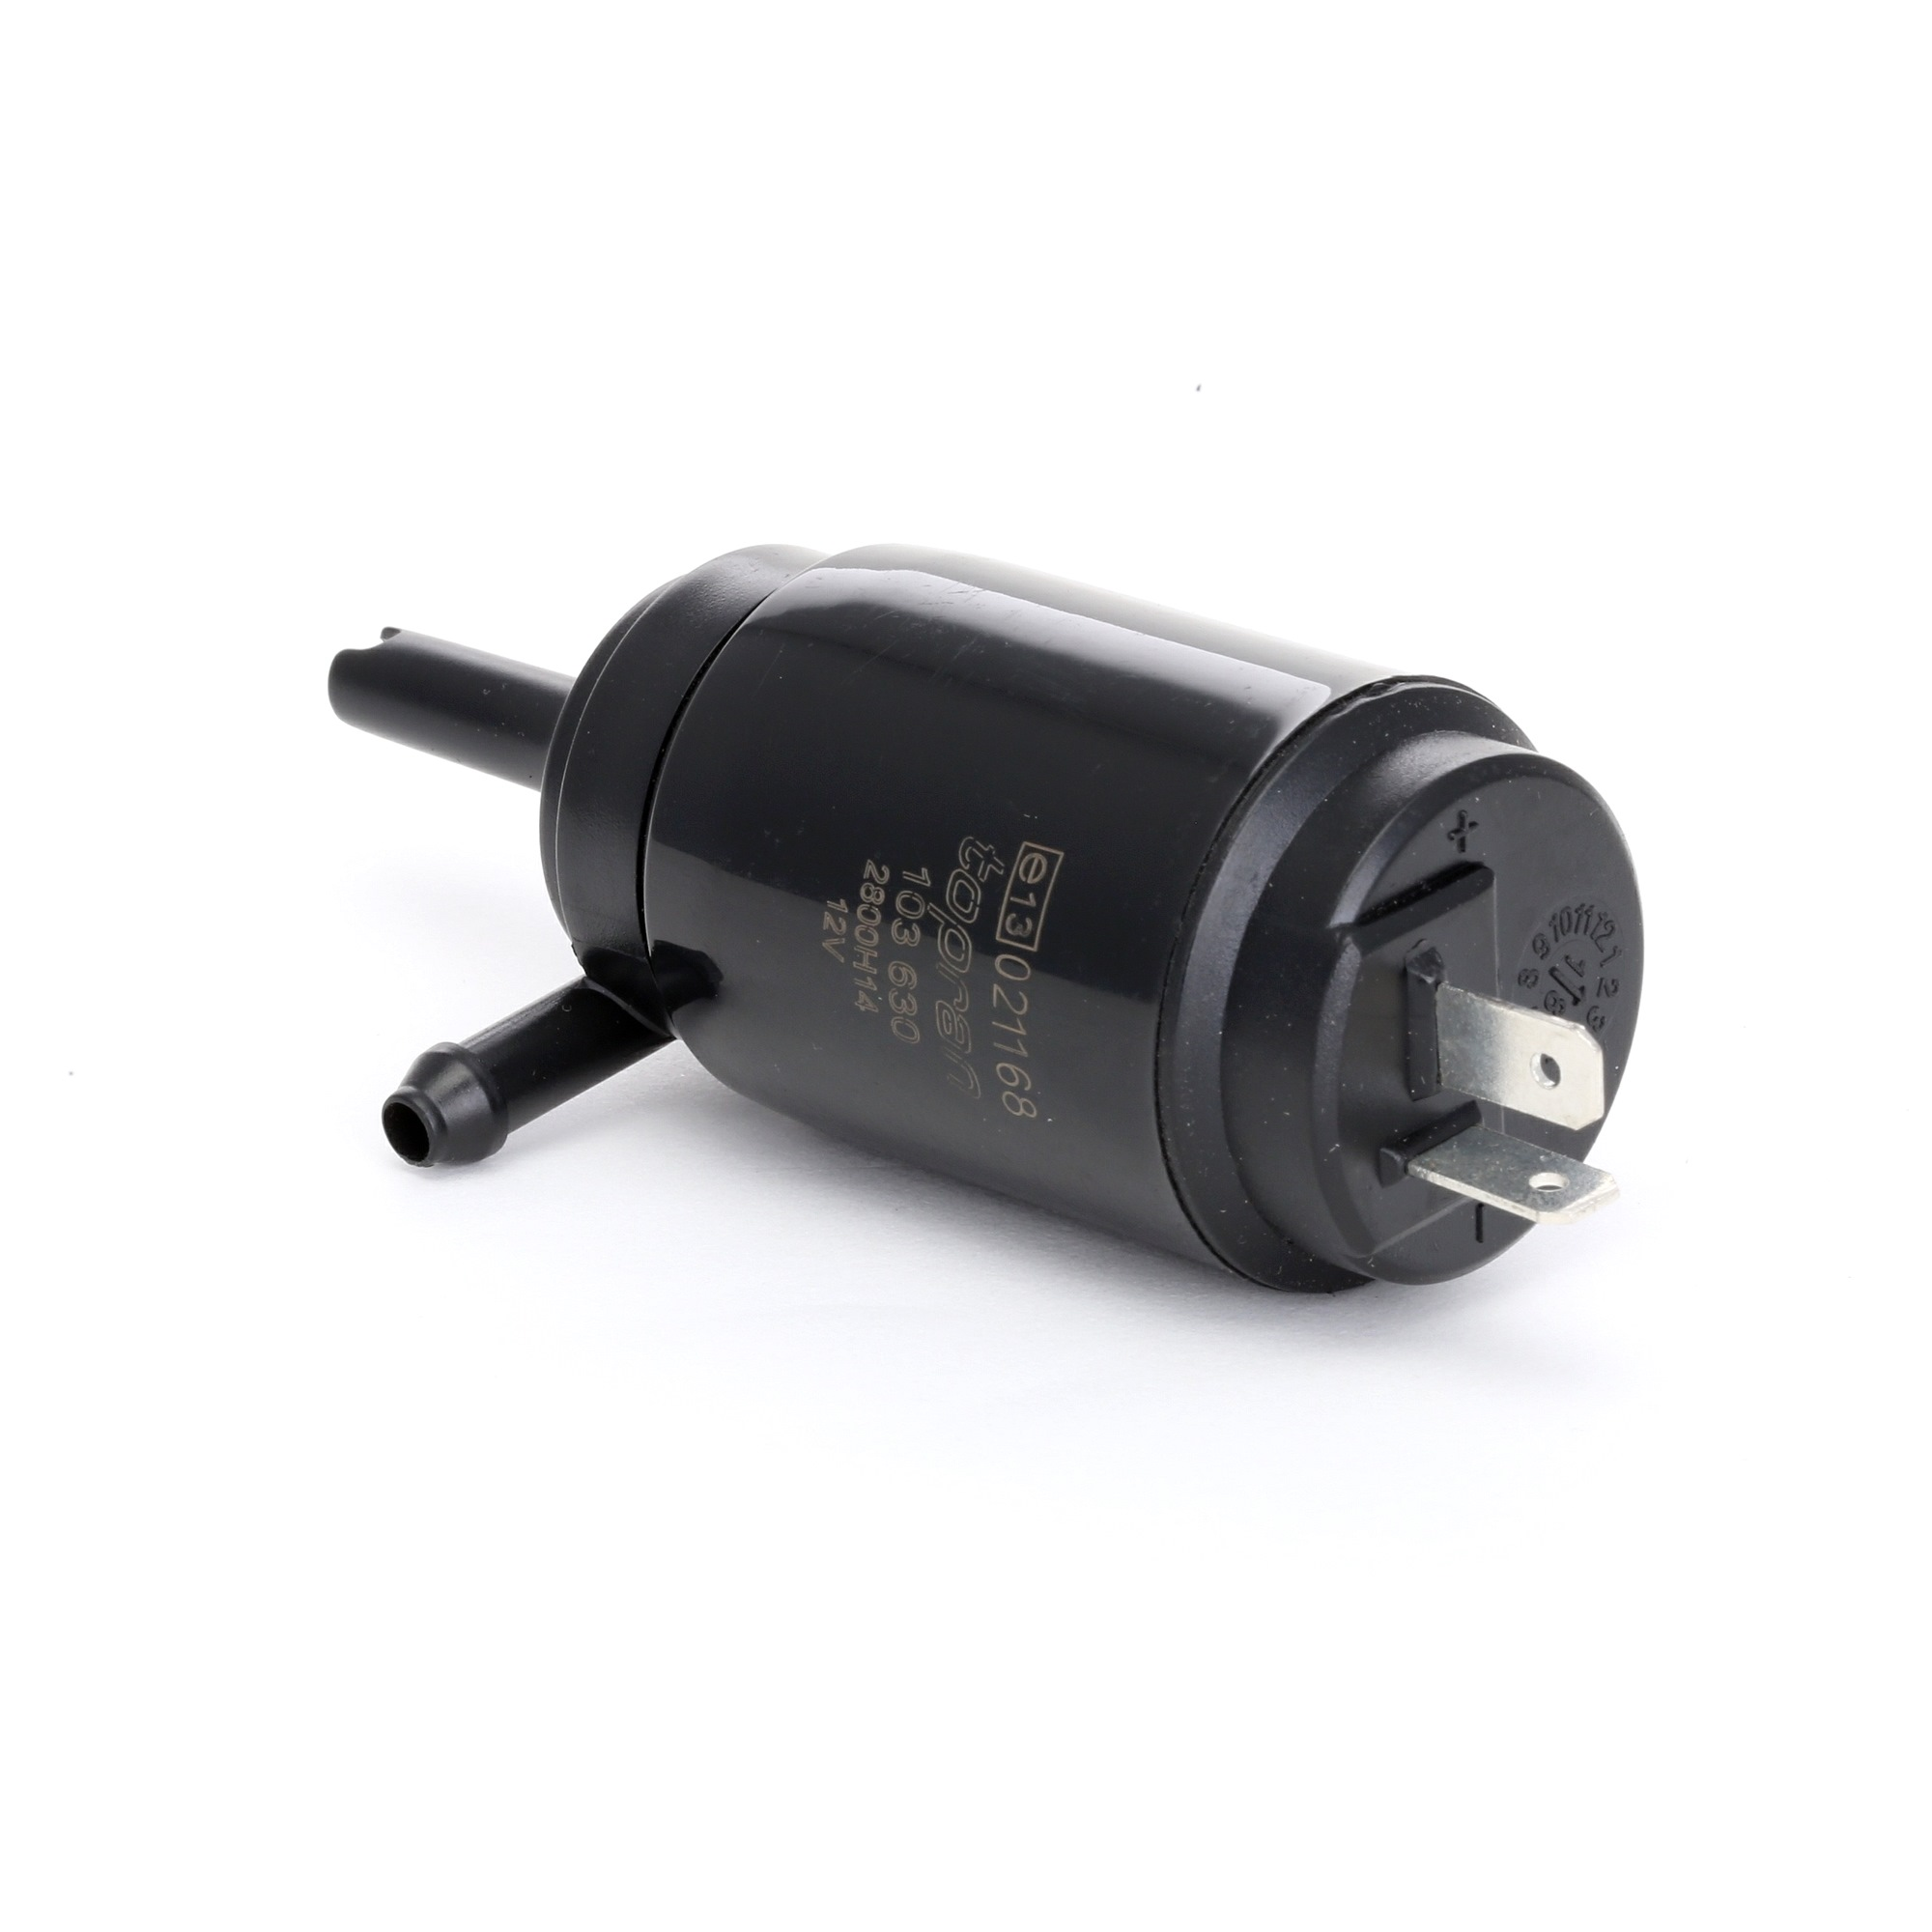
\includegraphics[width=0.4\textwidth]{pompka_photo.png}}
%\quad
%\subfloat[Bateria 9V~\cite{bateria}]{\label{odnosnik}
%
\includegraphics[width=0.4\textwidth]{9v.jpg}}
%\caption{Komponenty pompki}
%\label{fig:komponenty}
%
%\end{figure}
%
%
%
%\newpage
%\subsubsection{Obudowa}
%Obudowa na komponenty naszego projektu została zaprojektowana w programie Fusion360. Model ten został ''pocięty'' (przygotowany do druku) przy użyciu programu Cura i wydrukowany na drukarce 3D Ultimaker 2+. Został użyty materiał do drukowania o nazwie PLA (Polilaktyd) i dysza drukująca wielkości 0.8mm, co jak na standardy drukowania 3D jest dosyć dużo, jednak nie była wymagana duża dokładność. Prędkosć drukowania elementów była ustawiona na 40 [mm/s] i chłodzenie na 100 [\%]
%Czas drukowania pokrywki i pudełka wyniósł 12 godzin, nie licząc nieudanych druków i czasu spędzonego na dostrajanie drukarki.
%Model obudowy przedstawiony na Rysunku nr \ref{fig:modelobudowy}.
%\begin{figure}[!h]
%	\begin{center}
%		{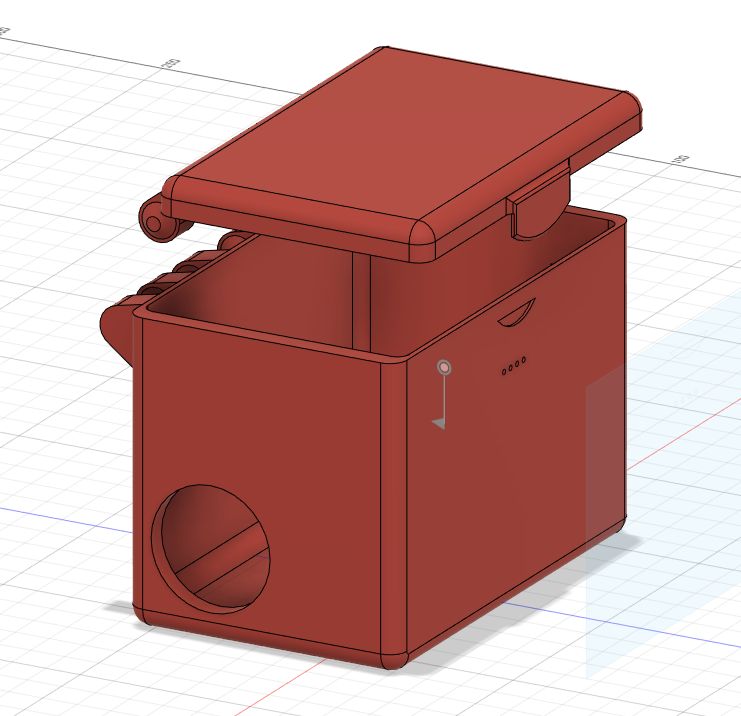
\includegraphics[width=9cm]{obudowa_model.png}}
%	\end{center}
%	\caption{Model obudowy (Fusion360)}
%	\label{fig:modelobudowy}
%\end{figure}
%
%\newpage
%\subsection{Szczególne rozwiązania warstwy programowej}
%\subsubsection{Płytka rozwojowa UNO}
%Realizacja oczekiwania płytki rozwojowej UNO na sygnał sterujący z ESP8266 została wykonana poprzez ciągłe sprawdzanie czy jej bufor przechowuje jakąś informację. Gdy wykryjemy, że bufor nie jest pusty to zczytujemy jego zawartość. Dane, które są odbierane będą zawarte we wskaźnikach początku ''<'' i końca ''>'' danej komendy. Dzięki temu rozwiązaniu możemy wykryć kiedy zaczyna się nowa instrukcja i wyczyścić pozostałości, jakie mogły pozostać w buforze, a także wykryć jej zakończenie. Zapobiega to "gubieniu danych" i otrzymywaniu powielonych instrukcji.
%
%Płytka rozwojowa UNO przedstawiona na Rysunku nr \ref{fig:uno}.
%\begin{spverbatim}
%	Część kodu płytki rozwojowej UNO odbierająca dane
%\end{spverbatim}
%\begin{lstlisting}
%while (Serial.available()) 
%{
%	char serialChar = Serial.read(); 
%	if (serialChar == '<')  
%	{
%		serialMessage = "";
%		serialMessage += serialChar;
%	}
%	else if (serialChar == '>')
%	{
%		stringComplete = true;
%		serialMessage += serialChar;
%	}
%	else
%	{ 
%		if ((serialChar >= 48 && serialChar <= 122) || serialChar == ',') 
%		serialMessage += serialChar;
%	}}
%	if( stringComplete == true)
%\end{lstlisting}
%
%
%\begin{figure}[!h]
%	\begin{center}
%		{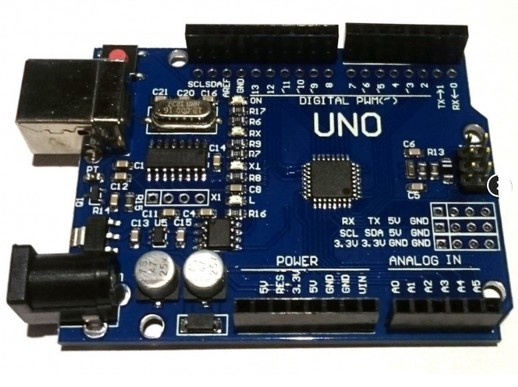
\includegraphics[width=7cm]{uno_photo.png}}
%	\end{center}
%	\caption{Płytka rozwojowa UNO}
%	\label{fig:uno}
%\end{figure}
%
%\newpage
%\subsubsection{ESP8266}
%Połączenie płytki ESP8266 z Internetem jest realizowane z pomocą biblioteki ESP8266WiFi.h, która ułatwia nam połączenie poprzez dodanie klasy WiFiClient przyjmującej argumenty nazwy sieci Wi-Fi i hasła oraz łączącej się automatycznie z Internetem.
%Będąc w tej samej sieci Wi-Fi, łączymy się z naszym serwerem na wcześniej zadeklarowanym IP i porcie za pomocą metody stworzonej z użyciem biblioteki WebSocketClient.h.
%Aby ułatwić testowanie, po każdym nieudanym połaczeniu restertujemy ESP, aby próbowało cały czas się połączyć.
%
%Tak jak w płytce rozwojowej UNO, odbieranie i wysyłanie danych jest realizowane we wskaźnikach początku ''<'' i końca ''>''.
%
%ESP8266 przedstawiona na Rysunku nr \ref{fig:esp}.
%\begin{figure}[!h]
%	\begin{center}
%		{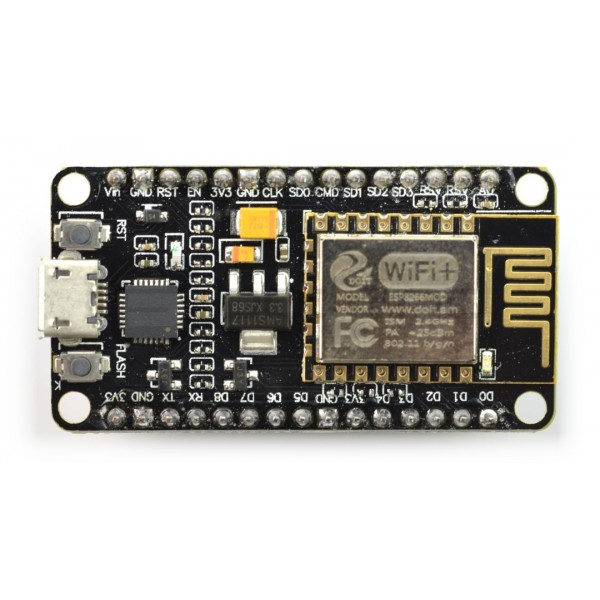
\includegraphics[width=12cm]{esp8266_photo.png}}
%	\end{center}
%	\caption{ESP8266}
%	\label{fig:esp}
%\end{figure}
%
%\newpage
%\subsubsection{Panel sterowania przez Internet}
%Panel sterowania został napisany z wykorzystaniem języka HTML i styli CSS wraz z różnego rozdaju frameworkami takimi jak Bootstrap. Zależało nam na prostocie, możliwości łatwej rozbudowy i szybkim dostępie do wszystkich potrzebnych parametrów danej roślinki. Pozwala on na sterowanie nawadnianiem i innymi, możliwymi do impementacji czynnościami poprzez kliknięcie przycisku na stronie z nazwą funkcji nawet przez osoby, które z internetem mają mało wspólnego.
%
%
%Dzięki skryptom, strona automatycznie pobiera informacje z płytki ESP8266, obrazuje je w postaci tabeli, a następnie tworzy wykres w oparciu o wszystkie zebrane dotychczas dane. Wstępny okres między aktualizacjami wynosi 5 sekund, jednak w razie zaistniałej potrzeby jest możliwość bardzo łatwej zmiany tego parametru nawet w edytorze tekstowym. 
%
%Panel sterowania przedstawiony na Rysunku nr \ref{fig:panel} wraz z przykładowymi pomiarami.
%\begin{figure}[!h]
%	\begin{center}
%		{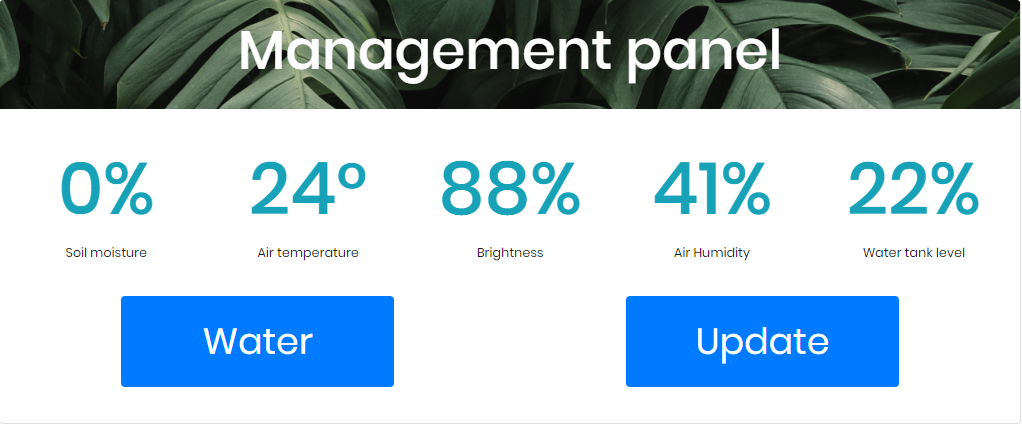
\includegraphics[width=16cm]{front panel.png}}
%	\end{center}
%	\caption{Panel sterowania}
%	\label{fig:panel}
%\end{figure}
%
%\newpage
%
%\section{Realizacja projektu}
%\subsection{Problematyka projektu}
%Przed rozpoczęciem prac nad projektem utworzyliśmy tabele w programie internetowym Trello, na których zapisaliśmy rzeczy potrzebne do zrobienia, a także podział kto jakimi elementami projektu się zajmie. Najtrudniejszą częścią wydawała nam się implementacja połączeń pomiędzy płyką rozwojową UNO, ESP8266 oraz serwerem, więc postanowiliśmy zacząć od tego, a dopiero później przejść do następnych aspektów. Wyzwaniem dla nas była również współpraca nad tak rozległym projektem, w którym wymagane było poprawne i integralne działanie zarówno części hardware'u, jak i tej internetowej. Zdecydowanie z pomocą przyszedł nam GitHub, ułatwiający zarówno równoległą pracę, jak i ewentualne poprawy błędów. 
%
%\subsection{Sposób wykonania}
%
%
%Postanowiliśmy połączyć płytkę rozwojową UNO obsługującą pompkę i monitorującą wartości naszych czujników z ESP8266, aby była możliwość sterowania poprzez Internet.
%
%Płytka rozwojowa UNO cały czas oczekuje na przychodzące dane które będą zawarte we wskaźnikach początku ''<'' i końca ''>'' danej komendy, aby wykonać określoną czynność lub odesłać pomiary wykonane przez czujnik wilgotności i temperatury do ESP8266, które jest połączone z UNO poprzez piny RX i TX. UNO odsyła swoje komendy również w wskaźnikach początku i końca, aby zapobiec ''gubieniu'' danych.
%
%ESP8266 jest naszym tzw. ''mostem'' i w każdym momencie czeka na dane czy to z UNO czy ze strony internetowej i w zależności od kogo dane otrzymuje przerzuca je do danego odbiorcy.
%Program na ESP jest zrealizowany z użyciem bibliotek ESP8266WiFi, WebSocketClient, SoftwareSerial, które kolejno służą do: umożliwieniu połączenia się ESP do sieci WiFi zadeklarowanej w naszym kodzie, połączeniu się poprzez websocket jako klient do naszego serwera postawionego na laptopie, połączenia się poprzez wyprowadzenie RX i TX do płytki rozwojowej UNO.
%
%Serwer do którego łączy się ESP8266 działa na laptopie. Połączenie jest realizowane z użyciem websocketów. Dzięki takiemu rozwiązaniu możemy wpisać adres na którym działa nasz serwer do przegladarki i ujrzeć stronę pozwalającą na kontrolowanie naszego urządzenia. Sterowanie odbywa się za pomocą przycisków umieszczonych na głównym panelu, które po naciśnięciu wysyłają daną komendę do podłączonych klientów - w tym przypadku naszego ESP8266. Dane pomiarowe przychodzące do serwera są zapisywane w stworzonej na potrzeby projektu bazie danych i przedstawiane graficznie w postaci wykresów na stronie.
%
%\newpage
%\subsection{Problemy napotkane podczas realizacji}
%\subsubsection{Połączenie między UNO, a ESP8266}
%Próbowaliśmy różnych typów połączeń jak I2C, albo SPI jednak poprawność testowych danych jakie otrzymywaliśmy była nikła - albo dostawaliśmy tylko część danych, albo były one w różny sposób powielone.
%Rozwiazaliśmy ten problem poprzez użycie wskaźników początku ''<'' i końca ''>'' przy wysyłaniu danej komendy, aby wykonać określoną czynność lub odesłać pomiary. 
%\subsubsection{Projektowanie i drukowanie obudowy}
%Dużym problemem była niewiedza związana z rozmiarem, jaki powinna mieć obudowa, jednak zdecydowaliśmy, że będzie ona większa niż nasze potrzeby, aby umożliwić łatwe rozbudowanie projektu w przyszłości. 
%
%
%
%Przy początkach drukowania popełniliśmy błąd złej początkowej wysokości druku co spowodowało że model był drukowany w powietrzu a co za tym idzie druk się nie powiódł. Kalibracja drukarki 3D naprawiła nasz problem i druk został wykonany poprawnie
%
%Nieudany druk pokrywki przedstawiony na Rysunku nr \ref{fig:drukfailed}.
%\begin{figure}[!h]
%	\begin{center}
%		{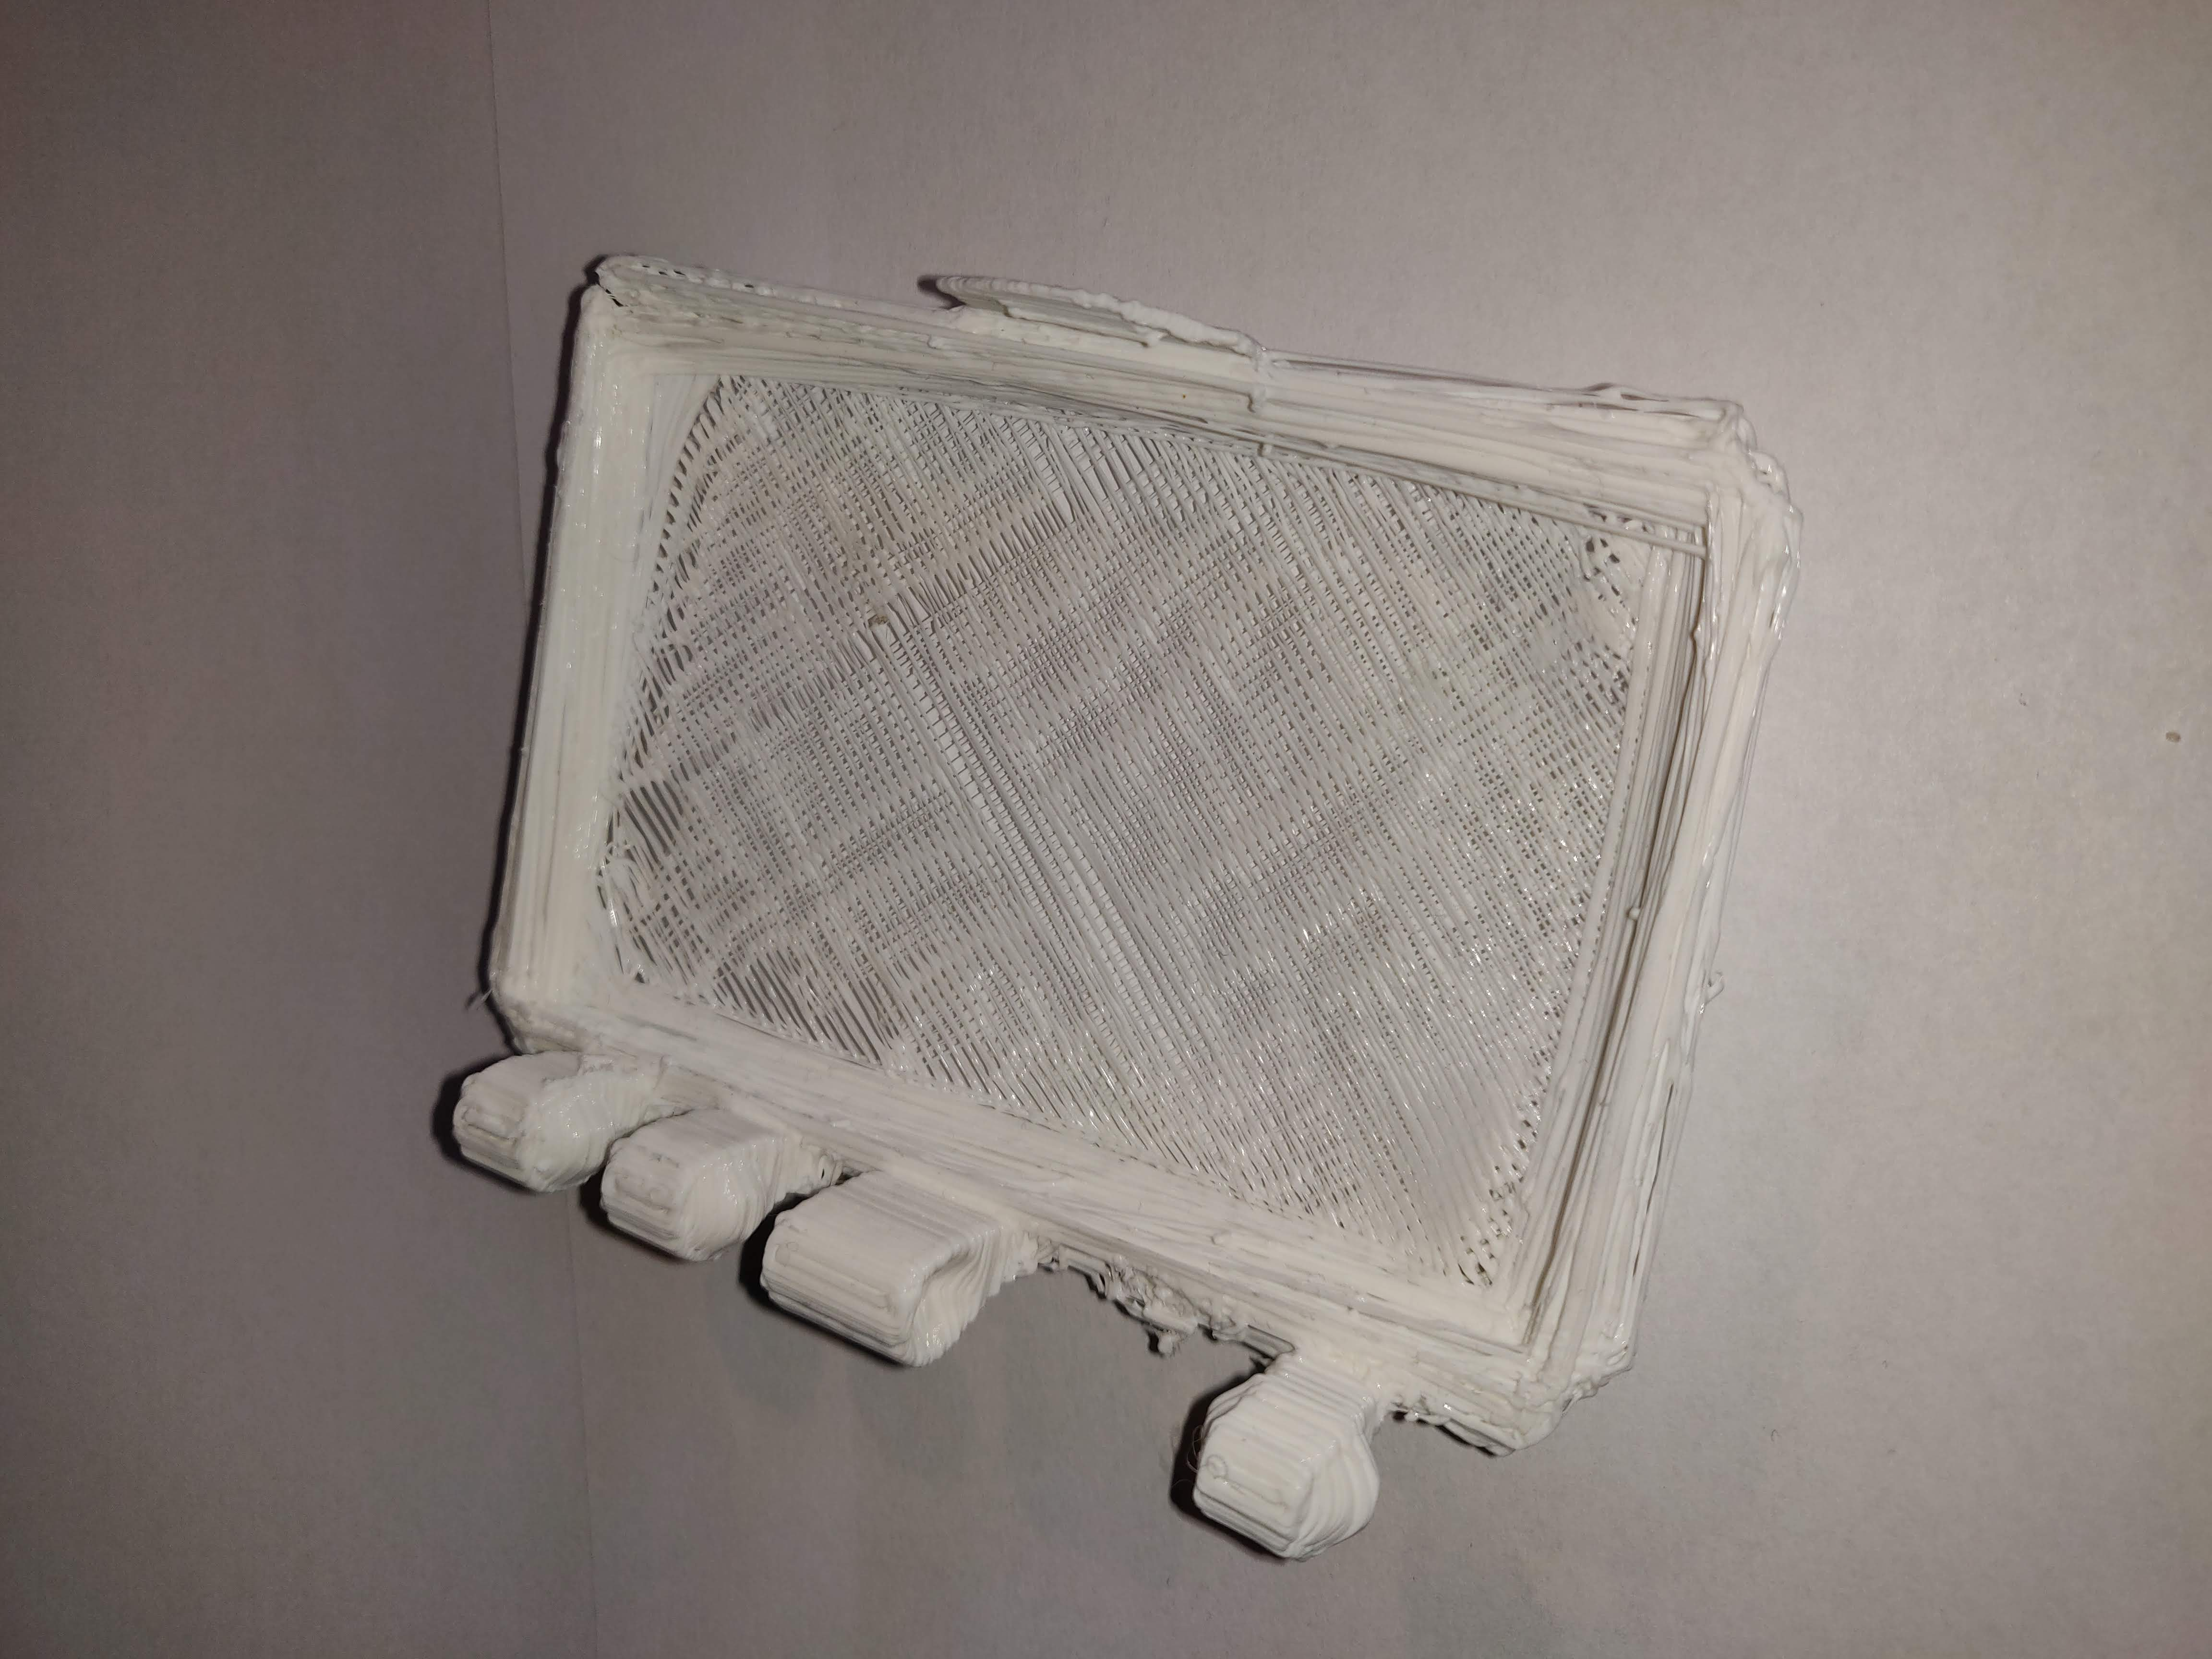
\includegraphics[width=12cm]{obudowa_broken.jpg}}
%	\end{center}
%	\caption{Nieudany druk pokrywki}
%	\label{fig:drukfailed}
%\end{figure}
%
%\newpage
%\section{Harmonogram i podział obowiązków}
%
%\subsection{Podział obowiązków}
%Kamil zajął się:\\
%- Uruchomieniem i szczegółowym zaznajomieniem się z plytką UNO wraz z modułem ESP8266,\\
%- Testowaniem i implementacją czujników oraz innych komponentów elektrycznych,\\
%- Implementacją połączenia między płytką rozwojową, a ESP8266,\\
%- Zaprojektowaniem ułożenia elementów na płytce PCB wraz ze stworzeniem obudowy metodą druku 3D,\\
%- Przeniesieniem projektu na płytkę  i włożeniem do obudowy\\
%
%Oskar zajął się:\\
%- Dostarczeniem potrzebnych materiałów i komponentów,\\
%- Stworzeniem serwera i panelu sterowania,\\
%- Implementacją połączeń między ESP8266, a serwerem,\\
%- Stworzeniem bazy danych wraz z graficznym przedstawieniem odczytów,\\
%- Testowaniem
%
%\subsection{Wstępny schemat blokowy}
%Przed rozpoczęciem pracy nad projektem stworzyliśmy schemat za pomocą programu draw.io, którego staraliśmy się trzymać, jednak ze względu na pewne komplikacje w trakcie realizacji pewne aspekty zostały zmienione, co zostało przedstawione na finalnym schemacie blokowym.
%
%Wstępny schemat blokowy przedstawiony na Rysunku nr \ref{fig:wstepnyschemat}.
%\begin{figure}[!h]
%	\begin{center}
%		{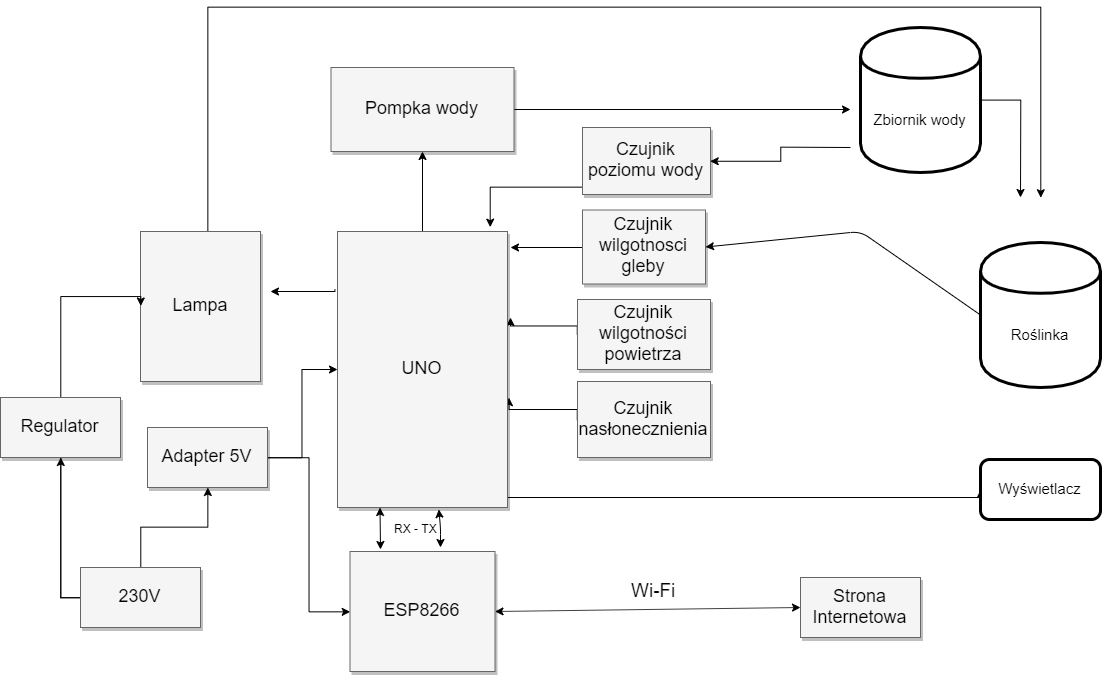
\includegraphics[width=14cm]{schemat_blokowy.png}}
%	\end{center}
%	\caption{Wstępny schemat blokowy}
%	\label{fig:wstepnyschemat}
%\end{figure}
%
%\newpage
%\subsection{Końcowy schemat blokowy}
%Można zauważyć, że nasz schemat zmienił się, jednak różnice nie są duże, a koncepcja projektu została zachowana. Zmiany zostały wprowadzone w trakcie budowy projektu ze względu na problemy z implementacją oświetlenia, a także poprzez decyzję o zasilaniu pompki wodnej z użyciem baterii 9 [V], gdyż płytka rozwojowa UNO nie była w stanie dostarczyć dostatecznie dużego natężenia prądu.
%
%Końcowy schemat blokowy przedstawiony na Rysunku nr \ref{fig:koncowyschemat}.
%\begin{figure}[!h]
%	\begin{center}
%		{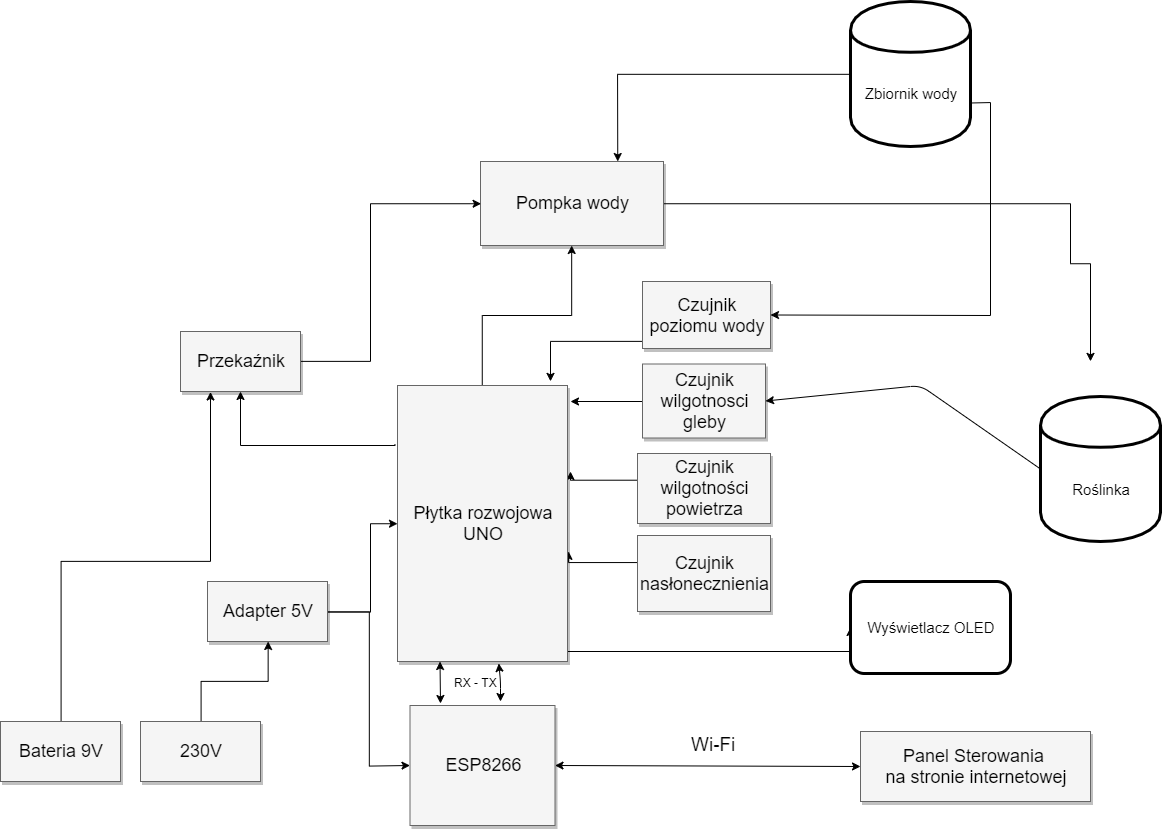
\includegraphics[width=16cm]{schemat_blokowy_koncowy.png}}
%	\end{center}
%	\caption{Końcowy schemat blokowy}
%	\label{fig:koncowyschemat}
%\end{figure}
%
%\newpage
%\subsection{Schemat elektryczny}
%Z użyciem programu EasyEDA został utworzony schemat elektryczny projektu.
%Schemat elektryczny przedstawiony na Rysunku nr \ref{fig:elekschemat}.
%\begin{figure}[!h]
%	\begin{center}
%		{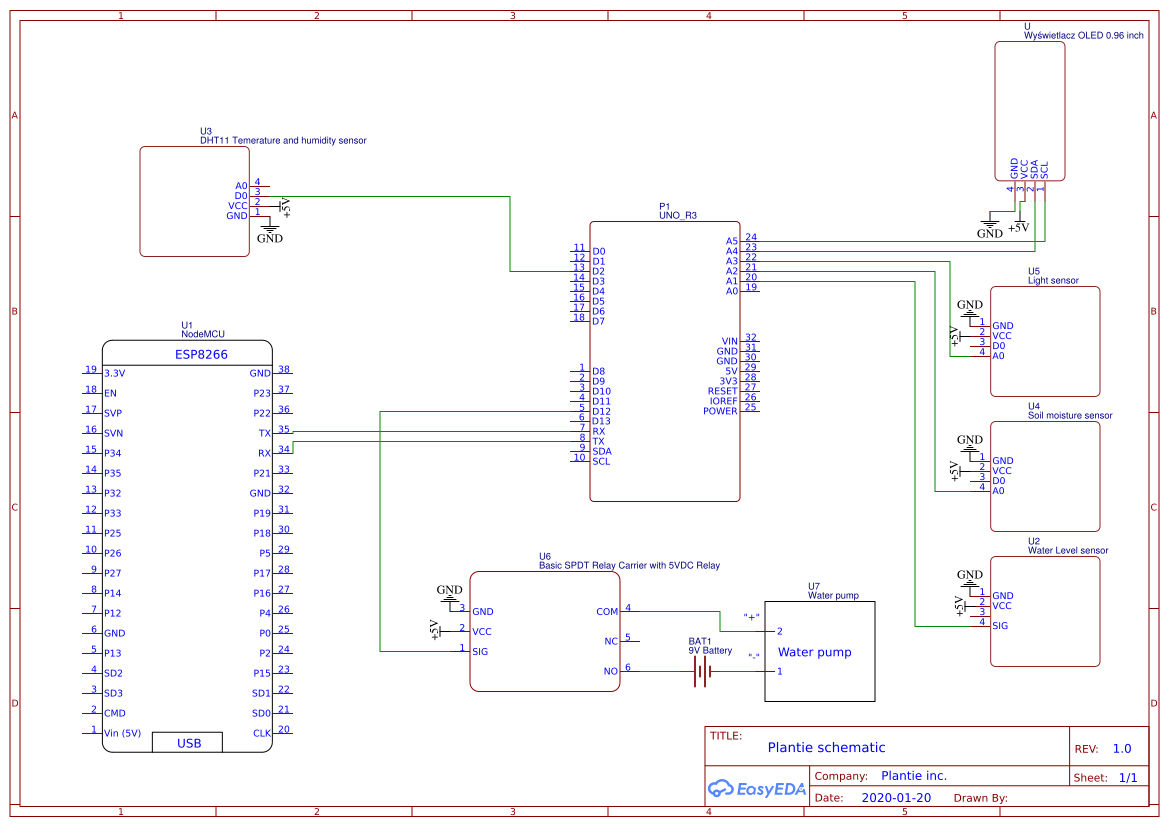
\includegraphics[width=17cm]{schemat_elek.png}}
%	\end{center}
%	\caption{Końcowy schemat blokowy}
%	\label{fig:elekschemat}
%\end{figure}
%
%
%\newpage
%\subsection{Harmonogram}
%\subsubsection{4.11}
%Przeanalizowanie schematów płytki rozwojowej UNO, modułu komunikacyjnego ESP8266, czujnika wilgotności gleby, czujnika wilgotności powietrza, czujnika nasłonecznienia oraz rozwiązanie techniczne doświetlania rośliny. Stworzenie schematu elektrycznego gotowego projektu. Testowanie poprawności działania posiadanych czujników w warunkach domowych. Implementacja komunikacji z modułem ESP8266. Dopasowywanie czasów działania. 
%Dokupienie brakujących komponentów gotowego projektu. 
%\subsubsection{25.11}
%Realizacja połączeń elektrycznych na płytce stykowej i ostateczne testowanie poprawności dzia-
%łania. Przeniesienie projektu na płytkę uniwersalną. Przygotowanie ewentualnej obudowy i realiza-
%cja montażu systemu doświetlania. Stworzenie prezentacji na zajęcia
%
%\subsubsection{16.12}
%Wstępna prezentacja gotowego projektu i ocena błędów.
%
%\subsubsection{20.01}
%Ostateczna prezentacja z poprawką błędów.
%
%\newpage
%
%\subsection{Zgodność z harmonogramem}
%Okazało się, że założony harmonogram był zbyt optymistyczny. Założyliśmy zbyt wiele rzeczy do zrobienia w początkowej części harmonogramu, a nie ustaliliśmy dużo na końcową część, jednak dzięki temu mieliśmy czas na dokończenie zaplanowanych aspektów projektu i nie przekroczeniu danego czasu na ukończenie go.
%
%\subsubsection{4.11}
%Rozpoczęliśmy prace nad projektem. Postanowiliśmy skorzystać z aplikacji internetowej Trello do utworzenia tabel, które umożliwiły lepsze zarządzanie podziałem prac.
%
%Przeanalizowaliśmy schematy płytki rozwojowej UNO, modułu komunikacyjnego ESP8266, czujnika wilgotności gleby, czujnika wilgotności powietrza oraz czujnika nasłonecznienia. Przetestowaliśmy również działanie każdego z czujników poprzez wykonanie przykładowych kodów na płytce rozwojowej UNO. Dowiedzieliśmy się, jakich komponentów projektu nam brakuje i zamówiliśmy je w wybranych sklepach.
%Stworzyliśmy wstępny schemat blokowy projektu, aby ukazać działanie poszczególnych elementów zawartych w naszym projekcie. Na ten moment postanowiliśmy nie tworzyć schematu elektrycznego, gdyż nie wiedzieliśmy jak dokładnie zrealizujemy poszczególne połączenia.
%
%Ze względu na obszerność testowania i planowanie realizacji planu działania na nadchodzące tygodnie, nie zajęliśmy się komunikacją z modułem ESP8266  ani problemem związanym z doświetlaniem rośliny.
%
%
%\subsubsection{25.11}
%Do tego dnia zajmowaliśmy się komunikacją między płytką rozwojową UNO, ESP8266, a stroną internetową. Napotkaliśmy wiele problemów co nieplanowanie wydłużyło nam pracę na tym etapie projektu. Udało nam się uzyskać stabilne połączenie między naszymi urządzeniami. Zrealizowaliśmy połączenia UNO, ESP8266, a także podłączyliśmy do układu czujnik wilgotności i temperatury powietrza i na płytce stykowej po czym przetestowaliśmy poprawność działania. 
%
%Przeniesienie projektu na płytkę uniwersalną okazało się niepraktyczne na tym etapie projektu, gdyż nie próbowaliśmy jeszcze połączyć ze sobą wszystkich modułów projektu i finalny kod do wgrania na UNO i ESP8266 nie był gotowy. Z powodu niewiedzy jak dokładnie będzie wyglądało nasze urządzenie na płytce uniwersalnej nie przygotowaliśmy planowanej obudowy. Nie zrealizowaliśmy również systemu doświetlania.
%
%\subsubsection{16.12}
%Podłączyliśmy ze sobą wszystkie czujniki na płytce uniwersalnej i testowaliśmy poprawność działania. Zajęliśmy się projektowaniem obudowy w programie Fusion360, abyśmy mogli ją wydrukować na drukarce 3D i włożyć do obudowy komponenty naszego projektu. Wydrukowaliśmy obudowę i wsadziliśmy tam wszystkie moduły projektu.
%
%\subsubsection{20.01}
%Stworzyliśmy techniczno-reklamową prezentację projektu, a także rozległy raport końcowy. 
%
%
%\newpage
%\section{Podsumowanie }
%\subsection{Osiągnięte cele}


%Ku naszemu zdziwieniu, projekt zajął zdecydowanie więcej czasu niż mogliśmy się spodziewać. Brak wiedzy skutkował tym, że nie wiedzieliśmy nawet gdzie i czego szukać. Na szczęście internet w dzisiejszych czasach jest bardzo obszerny w różnego rodzaju poradniki i źródła, które pomogły nam zrealizować cele i wyjaśnić czemu poprzednie próby musiały zakończyć się fiaskiem. 
%
%Podsumowując, jesteśmy bardzo zadowoleni z ogólnego rezultatu. Niestety, nie wszystko poszło zgodnie z planem, lecz połączenie rozwiązań technicznych i cyfrowych oraz sprawienie, by działały wspólnie spowodowały powstanie ciekawego dla nas projektu oraz zdobycie bardzo cennej wiedzy. Realizacja własnego projektu mikroprocesorowego, który zmusza do samodzielnego myślenia, swoboda w jego tworzeniu oraz doprowadzenie całości do finalnego produktu jest z pewnością bardzo satysfakcjonująca i pomimo czasu, który trzeba w to włożyc, powinno być ich więcej.
%\subsection{Pomysły na rozwój projektu}
%Pomysłów na dalszy rozwój projektu jest wiele, ponieważ w trakcie prac przychodziło nam do głowy ich dużo jednak postanowiliśmy je tymczasowo zignorować i spróbować zrealizować postawione przez nas na początku cele. Nie zrealizowaliśmy również jednego aspektu projektu co też stało się naszym planem na przyszłość. \\
%
%Oświetlenie roślinki przy wykryciu za małej ilości światła.\\
%	
%Automatyzacja procesu podlewania po odczytaniu ustawionej dolnej granicy czujnika wiglotności gleby.\\
%
%Aplikacja umozliwiająca podgląd parametrów roślinki i zdalne sterowanie.\\
%	
%Domena i działanie projektu w chmurze bez potrzeby włączania serwera na laptopie. Do tego było by potrzebne przeniesienie naszej bazy danych na bazę danych w chmurze (np. Azure), a także implementacja ESP8266 jako serwera.\\
%
%

\newpage
\begin{thebibliography}{9}



\bibitem{Trutina} Trutina z Gremon Systems
gremonsystems.com/blog-en/things-you-didnt-know-about-automatic-watering-systems/

\bibitem{ArduinoIS} Arduino Irrigator System
http://www.circuitstoday.com/arduino-irrigation-plant-watering-using-soil-moisture-sensor

%
%
%\bibitem{latexcompanion} 
%Ivan Grokhotkov
%\textit{ESP8266 Arduino Core’s documentation}. 
%2017
%
%\bibitem{latexcompanion} 
%Christian Klippel, Peter Andersson, Peter Lerup
%\textit{ESP8266 core for Arduino}. 
%2017
%
%\bibitem{latexcompanion} 
%
%\textit{w3schools.com}. 
%1999-2019
% 
%\bibitem{przekaznik} Relay Module
%\emph{}
%opencircuit.shop
%
%\bibitem{pompka} Pompa spryskiwacza TOPRAN
%\emph{},
%www.autoczescionline24.pl/topran-2723484.html
%
%\bibitem{pompka} Dokumentacja ArduinoIDE 
%\emph{},
%forum.arduino.cc
%
%\bibitem{pompka} Testowanie obwodów elektrycznych 
%\emph{},
%www.circuitlab.com
%
%\bibitem{bateria} Bateria alkaliczna 9V 
%\emph{VARTA},
%elfadistrelec.pl/pl/alkaliczne-bateria-alkaliczna-9v-6lr61-varta-industrial-9v/p/16901614




\end{thebibliography}


\end{document}
